
\begin{enumerate}
    \item \textit{Risk-averse Two-stage Stochastic Programming for Distribution Grid Resilience:} The two-stage stochastic programming problem is formulated as a MILP problem where Stage-1 decisions are the infrastructure planning decisions optimized to reduce the risks of outages due to HILP events assuming optional operational phase decisions.
    \item \textit{Probabilistic scenario generation and smart scenario reduction strategy:} A Monte-Carlo-based probabilistic scenario generation framework and smart scenario selection strategy is proposed to reduce the large scenario samples to representative scenarios.
    \item \textit{Trade-off analysis on risk minimization vs. expected loss minimization:} Different case studies are presented to identify the trade-off of adopting risk-neutral vs. risk-averse policies in the planning decisions. The analysis can provide insights into adopting risk-driven solutions when the utmost priority is to maintain an uninterruptible power supply to critical customers during extreme weather events.
\end{enumerate}

\subsubsection{Planning Problem Representation}

A power distribution network can be graphically represented as $G(V,E)$, where the vertices $V$ represent the buses or nodes while the distribution lines are represented by the edges $E$. The overall objective of the two-stage framework is to identify the first-stage optimal planning decisions that minimize the expected operational cost in the second stage. In this work, DG siting and sizing are the planning decisions whereas the second stage objective is to minimize the prioritized load loss once a scenario is realized. DGs with grid-forming inverters are assumed in this work. Such grid-forming DGs can be used for intentional islanding when some area of the distribution grid gets disconnected from the system due to an extreme event. 

The two-stage objective function is a random variable. Thus, determining the optimal planning decision is the problem of comparing random cost variables as a function of the planning cost and the operational cost. The overall problem is formulated as a risk-averse stochastic optimization problem in which the first stage problem minimizes the cost of planning and the weighted combination of the expected value and the $CVaR$ of the second stage problem. The second stage problem is the operational stage that minimizes the total prioritized loss of load for every scenario realization.
    
    \begin{figure}[t]
        \centering
%    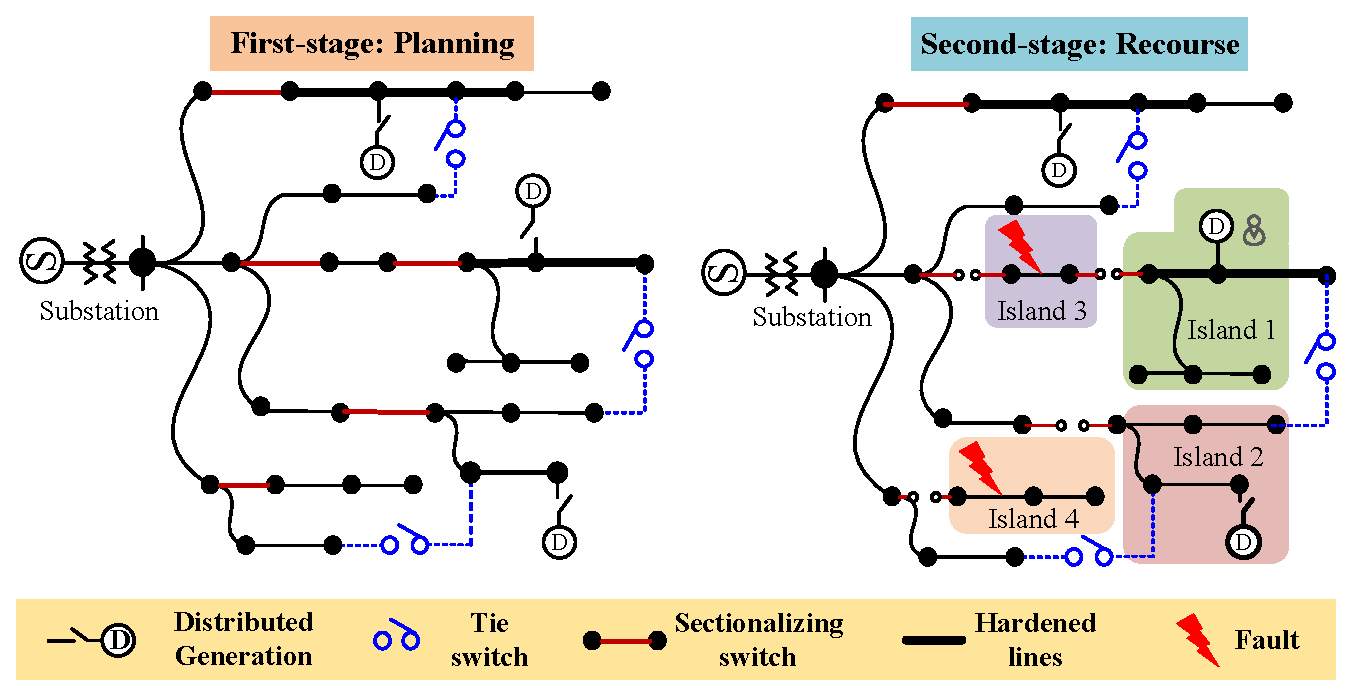
\includegraphics[width=0.75\textwidth]{figures/first_second_stage_model.eps}
        \caption{Two-stage planning framework example for a specific scenario.}
        \label{fig:model_representation}
    \end{figure}

\subsubsection{Problem formulation}
The resilience-driven distribution system planning problem is formulated as a two-stage stochastic optimization problem where the overall objective function can be defined as:

\begin{equation}
\small
    \begin{split}
    \min (1-\lambda)\mathbb{E}(Q(\delta, \mathcal{E})) + \lambda CVaR_\alpha(Q(\delta, \mathcal{E}))
    \end{split}
    \label{eq:main_objective}
\end{equation}
where,
\vspace{-5pt}
\begin{equation*}
\small
    \begin{gathered}
        \mathbb{E}(Q(\delta, \mathcal{E})) := \left(\sum_{\xi \in \mathcal{E}}\sum_{i\in  \mathcal{B}_S}\sum_{\phi\in\{a,b,c\}}(1 - s^\xi_i)\ w_i\ P_{Li}^{\phi,\xi}\right)\\
        CVaR_\alpha(Q(\delta, \mathcal{E})) := \left(\eta + \frac{1}{1-\alpha}\sum_{\xi \in \mathcal{E}}p^\xi\nu^\xi\right)
    \end{gathered}
\end{equation*}

The problem objective in the first stage is to minimize the weighted sum of expected value and $CVaR_\alpha$ of the second stage cost, represented by $Q(\delta, \mathcal{E})$. To analyze the trade-offs, this formulation has not used minimization of planning cost. Instead, we use a budget constraint and observe the associated trade-offs for risk-averse and risk-neutral decisions when system planners have a limited investment budget. The objective of the second stage of the problem, $Q(\delta, \mathcal{E})$, is to minimize the prioritized load loss or maximize the restoration of prioritized loads for each $\xi \in \mathcal{E}$. The second stage costs correspond to the optimal restoration decisions once a scenario has been realized. Hence, each variable corresponding to the second stage of the problem is scenario-dependent. $P_{Li}^{\phi,\xi}$ represents the active power demand at node $i$ for phase $\phi$ and scenario $\xi$ and $s_i^\xi \in {0, 1}$ is the load pick-up status variable that determines whether the load at node $i$ is picked up or not. The CLs are prioritized by a weight variable $w_i$. Since the CLs are critical for any scenario, $w_i$ remains the same for all scenarios. Furthermore, the scenarios have a specific probability, $p_\xi$, associated with them, which comes from the scenario reduction method discussed before. For the expression $CVaR_\alpha(Q(\delta, \mathcal{E}))$, $\nu_\xi$ is an excess variable which ensures that $CVaR_\alpha$ is calculated only for realizations beyond $VaR_\alpha$ for each scenario $\xi$. 

Here, DG location ($\delta^{DG}_i$) and size of the DG ($\beta^{DG}_i$) are the first stage decision variables. In this work, the per unit cost for DG installation and sizing is assumed to be the same for each location; these assumptions can be easily relaxed.  
Constraint (\ref{eq:DG_size}) ensures that the total cost of DGs should be between \$[0, $\mathcal{C}^{DG}_{max}$] regardless of the cost of installation in an individual location. This gives the freedom of utilizing the overall budget for a single big-sized DG or distributing the budget to multiple smaller-sized DGs. Constraint (\ref{eq:DG_size}) contains a non-linear term $\delta_i^{DG} \times \beta^{DG}_i$ which is linearized using big-M method as discussed in~\cite{coelho2013linearization}. Constraint (\ref{eq:DG_location}) restricts the DG location variable to binary. The DG location variable $\delta^{DG}_i$ is 1 if a DG is located in node $i$, else 0. Furthermore, constraint (\ref{eq:VAR_constraint}) ensures that $VaR_\alpha$ for the distribution of load loss in the second stage is a real number. Furthermore, $VaR_\alpha$ is independent of scenarios and is obtained with the solution of the first stage. 

\begin{subequations}
\begin{equation}
\small
    \sum_{i\in \mathcal{B}_{DG}} c_i^{DG}\delta_i^{DG} \beta^{DG}_i \leq \mathcal{C}^{DG}_{max} \\
    \label{eq:DG_size}
\end{equation}
\vspace{-10pt}
\begin{equation}
\small
    \delta^{DG}_i \in \{0,1\} \\
    \label{eq:DG_location}
\end{equation}
\begin{equation}
    \small
    \eta \in \mathbb{R} \\
    \label{eq:VAR_constraint}
\end{equation}
\end{subequations}

\noindent The overall problem formulation can be summarized as:\\
\newcommand\tab[1][0.5cm]{\hspace*{#1}}
	\tab Objectives:\\
	\tab \tab1) Minimize weighted sum of expected value and $CVaR_\alpha$ of the second stage cost\\
	\tab Constraints:\\
	\tab \tab1) First-stage constraints (scenario independent)\\
	\tab \tab2) Second-stage constraints (secenario dependent)\\
	\tab \tab \tab a) Connectivity constraints\\
	\tab \tab \tab a) Three-phase unbalanced power flow constraints\\
	\tab \tab \tab c) Network operational constraints\\
	\tab \tab \tab d) DG operating constraints\\
	\tab \tab \tab e) $CVaR_\alpha$ constraints

\subsubsection{Proposed scenario generation and selection approach}
The overall architecture of the proposed method is shown in Fig.~\ref{fig:overall_architecture}. Only wind-related events are used in this work and the probability distribution of extreme wind events is considered to generate the scenarios. Monte Carlo simulations (MCS) are conducted to identify the impact of probabilistic events, and an appropriate scenario reduction method is implemented to identify representative scenarios. Finally, the planning problem is solved in a two-stage stochastic optimization setting based on a selected number of scenarios.

\begin{figure}[t]
    \centering
%    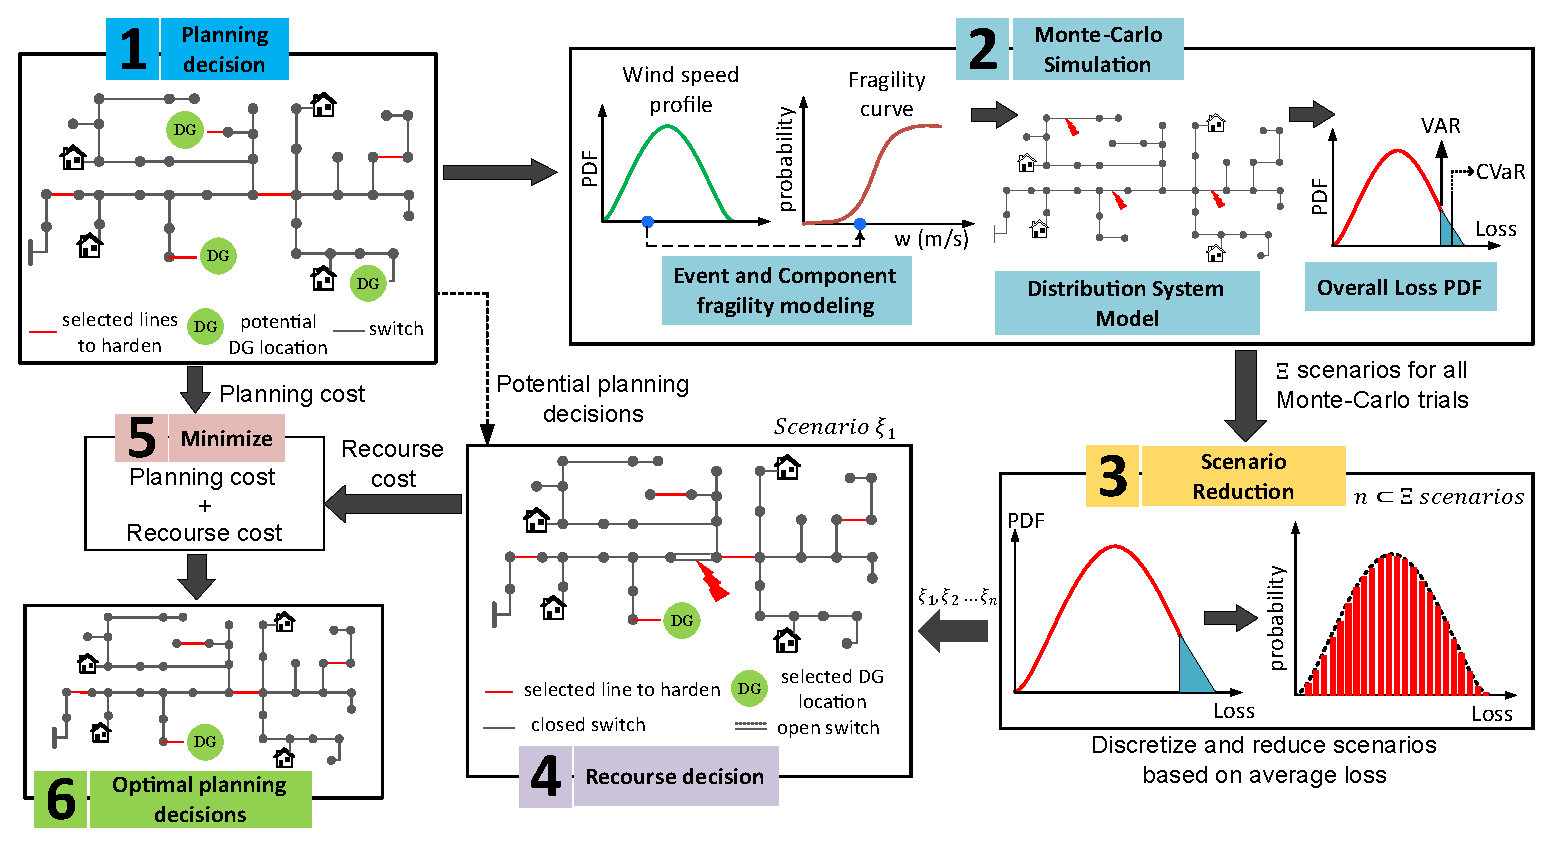
\includegraphics[width=0.8\textwidth]{figures/overall_picture.eps}
    \caption{Overall architecture of risk-averse two-stage planning problem. The first stage seeks the optimal planning decisions that minimize the expectation and risk of the recourse cost in the second stage for several scenario realizations. The scenarios are generated using Monte-Carlo simulation and reduced based on average loss for each scenario.}
    \label{fig:overall_architecture_framework}
\end{figure} 

\begin{figure}[h]
    \centering
%    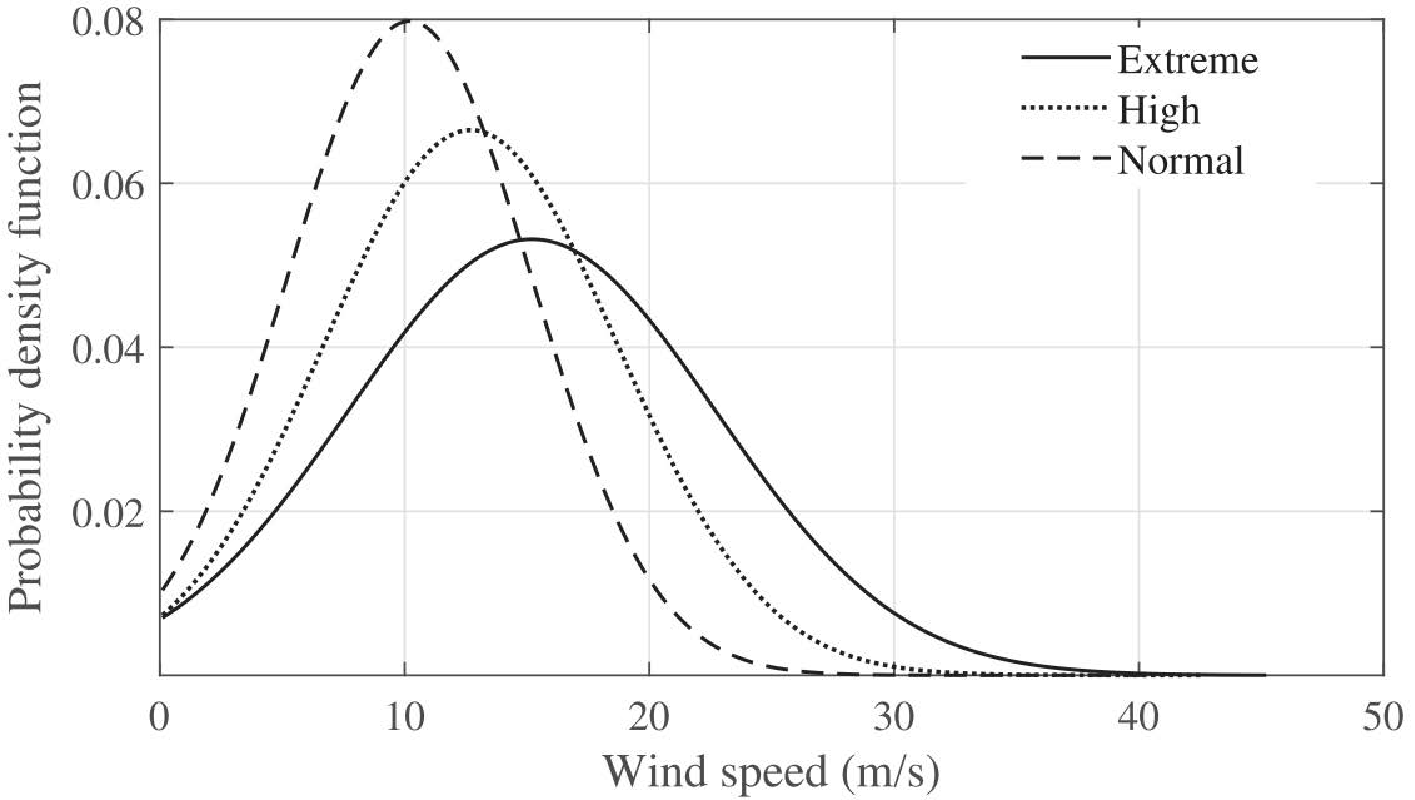
\includegraphics[width=0.7\textwidth]{figures/wind_profile.pdf}
    \caption{Regional wind profile.}
    \label{fig:wind_profile}
\end{figure}

Fig.~\ref{fig:wind_profile} shows the event probability distribution for a windfall in three different regions observing extreme, high, and normal wind profiles. The extreme regional wind profile is used to model extreme events in this work. For simplicity, only distribution lines are assumed to be affected by wind in this work. Although wind-related events have spatiotemporal dynamics~\cite{poudyal2021spatiotemporal}, we assume that for a distribution system, that covers a small region, the wind speed for the entire region is the same. MCS is performed for each wind speed case so as to also include the extreme tail probability events. This process is represented by block 2 in Fig.~\ref{fig:overall_architecture}. For each wind speed scenario $u$, the component level failure probability $p_f(u)$ determines the operational state of a particular component in the distribution grid. Component level fragility curves \cite{panteli2017power} or prototype curve fit models \cite{powell1995real} can be  used to model the impacts of extreme events such as hurricanes or other high-speed wind events on power systems. In this work, we have used the component fragility curve that maps the probability of failure of distribution system components conditioned on the intensity of the hazard (e.g., a wind speed). The fragility curve values are randomly selected for simulation purposes; however, if available, empirical data can be used to adjust the parameters~\cite{7036086}.

MCS provides an extremely large number of scenarios. One major challenge in any stochastic optimization setting is handling many scenarios within the optimization framework. Furthermore, the solution should be optimal for all scenarios that make the stochastic problem computationally intractable. Existing works use special sampling techniques such as stratified sampling~\cite{parsons2014stratified} or importance sampling~\cite{ekblom2020importance} to include the tail probability scenarios in the optimization model appropriately. Distance-based scenario reduction methods have also been used where a probabilistic distance measure is minimized to obtain a reduced scenario distribution that closely represents the overall scenario distribution~\cite{heitsch2007note}. We introduce a new approach to scenario reduction inspired by stratified sampling and distance reduction methods. The proposed approach uses stratification to sample representative scenarios for each wind speed and generates a reduced scenario distribution that closely matches the original scenario distribution.

In this work, the overall number of scenarios is reduced by selecting a representative scenario for each wind speed based on the average Monte-Carlo loss. This process is represented by block 3 in Fig. 3. Let $N_u$ be the total discrete wind speeds under consideration, $N_{\xi,u}$ be the number of scenarios obtained from MCS for each wind speed $u$, and $L^{u}_{avg} = \mathbb{E}(L_{\xi,u})$ be the average prioritized load loss in $kW$ corresponding to $N_{\xi,u}$ scenarios. Let $\Xi = N_{\xi,u} \times N_u$ be the total number of scenarios for the entire MCS. Note that we cannot randomly select a subset of these scenarios as it significantly degrades the accuracy of the optimization solutions. Here, we use a unique sampling technique to drastically reduce the number of scenarios while maintaining the representation of the overall scenarios described next. If $\xi_u$ is a representative scenario for all $N_{\xi,u}$ scenarios corresponding to $u$, then $\xi_u$ is selected such that the prioritized load loss in the system due to $\xi_u$ ($L^{u}_{\xi_u}$) is the one nearest to $L^{u}_{avg}$. In the case of multiple scenarios with losses nearing $L^{u}_{avg}$, one of the scenarios is randomly selected as $\xi_u$ from the identical scenario representations. The proposed scenario reduction technique reduces the total number of scenarios to $N_u$ from $\Xi$ such that $p_\xi$ corresponds to the wind speed profile. This smart scenario selection strategy ensures the practical realization of the second stage problem while incorporating HILP events within the scenarios. 

\subsubsection{Preliminary Research Results}
The effectiveness of the proposed risk-based long-term planning model is verified on a modified IEEE 123-bus case, see Fig.~\ref{fig:IEEE_123_testcase}. To analyze the planning decisions better, we create a new test case upon hardening 15 randomly selected lines, as shown in Fig.~\ref{fig:IEEE_123_testcase}. The fragility curves of hardened lines are adjusted so that their outage probability for any extreme event is less than the case when they are not hardened. For CLs, $w_i = 10$ whereas, for non-critical loads, $w_i = 1$. Thus the second stage cost reflects the total amount of prioritized loss of load (in kW). The total non-prioritized demand of the system is $P_D = 4485~kW$ and the prioritized demand is $\sum_{i\in\mathcal{V}}{w_iP_{Li}} = 20775~kW$. This work uses prioritized demand to analyze the results for different cases.

\begin{figure}[t]
    \centering
%    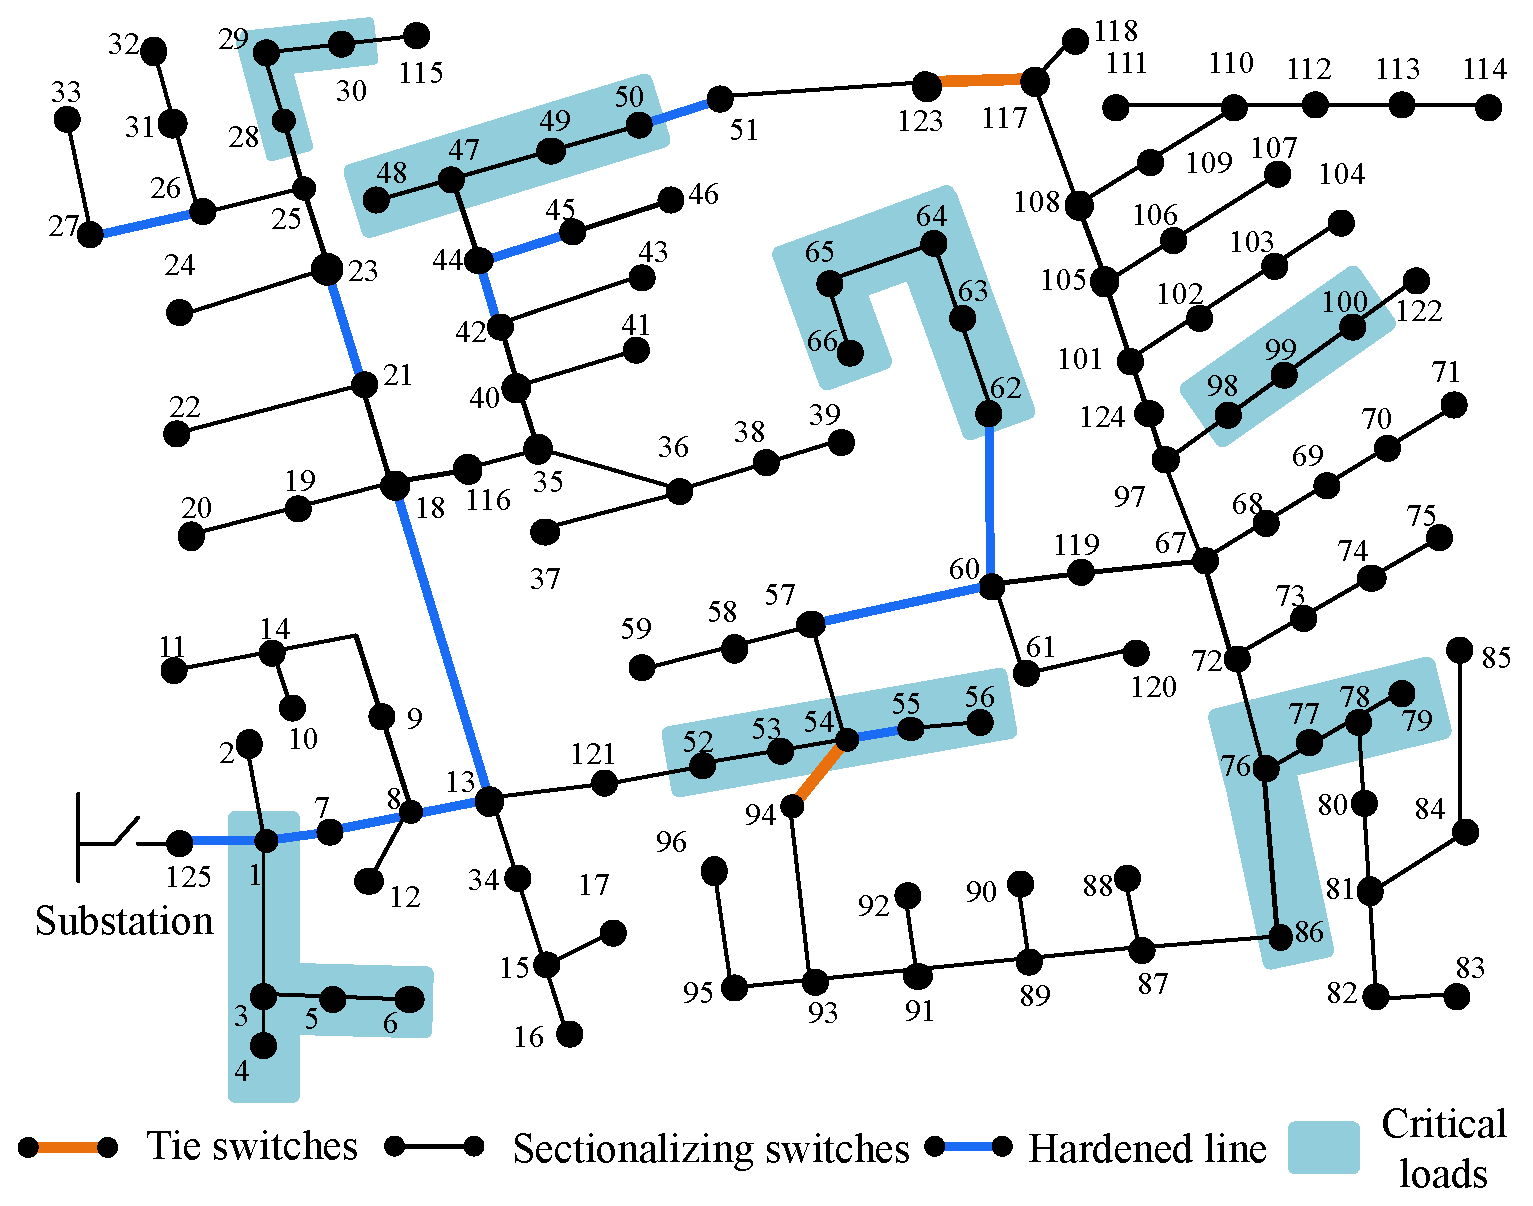
\includegraphics[width=0.7\textwidth]{figures/IEEE_123_CL_update.eps}
    \caption{Modified IEEE 123-bus test case}
    \label{fig:IEEE_123_CL_update}
\end{figure}

\paragraph{Scenario Generation and Reduction}
Using the wind speed profile for extreme wind events and failure probability of distribution lines, several trials of MCS simulation are conducted for sampled wind speeds~\cite{7036086}. For this experiment, $N_u=49$ wind speeds are sampled from the wind speed profile and it was experimentally verified that 1000 Monte-Carlo trials are enough to obtain a converged value of prioritized loss of load in the distribution grid corresponding to each $u$. Fig.~\ref{fig:MCS_convergence} shows the moving average of prioritized loss of load for 1000 Monte-Carlo trials for the base case without hardening and with hardening. It can be seen that the value of the loss is fairly converged in 1000 trials for both cases. Since 1000 trials are conducted for each $u$, $N_{\xi,u} = 1000$. Hence, the total number of scenarios generated through MCS, $\Xi = 49 \times 1000 = 49000$. 

Fig.~\ref{fig:scenario_reduction} represents the comparison between $L^u_{avg}$ and $L^u_\xi$ for the test case without hardening and with line hardening. The loss due to reduced scenarios is very close to that of the actual representative scenarios for each $u$. The y-axis on the right represents the value of $|L^u_{avg} - L^u_\xi|$. It can be seen that the maximum difference occurs at $u = 31 m/s$ in Fig.~\ref{fig:scenario_reduction}.a and has a value of about $78~kW$ which is $< 0.5\%$ of total prioritized demand. The difference in their values comes from the fact the $L^u_{avg}$ is obtained by averaging 1000 different realizations of $\xi$ for a specific $u$ whereas $L^u_\xi$ is the prioritized load loss for a specific failure scenario $\xi$ corresponding the same $u$. Furthermore, it should be noted that HILP events (tail events) are also sampled in this reduction method which makes this approach highly suitable for resilience planning problems.

\begin{figure}[t]
     \centering
    %  \subfigure[]
     {
%    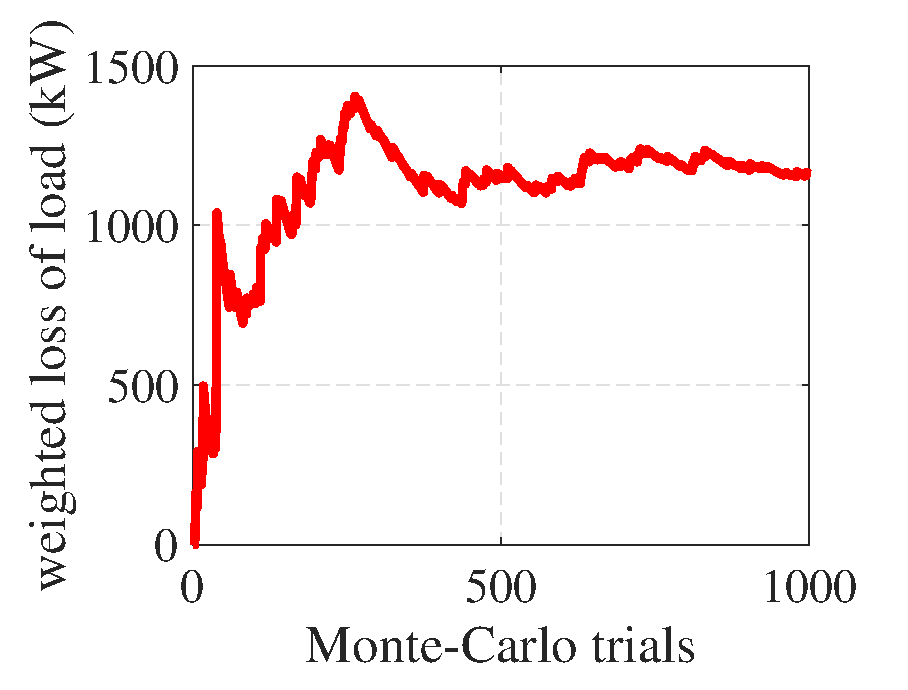
\includegraphics[width=0.42\linewidth]{figures/speed_15_MC_base.eps}
        \label{fig:MCS_1}
    }\hfill
    % \subfigure[]
    {
%    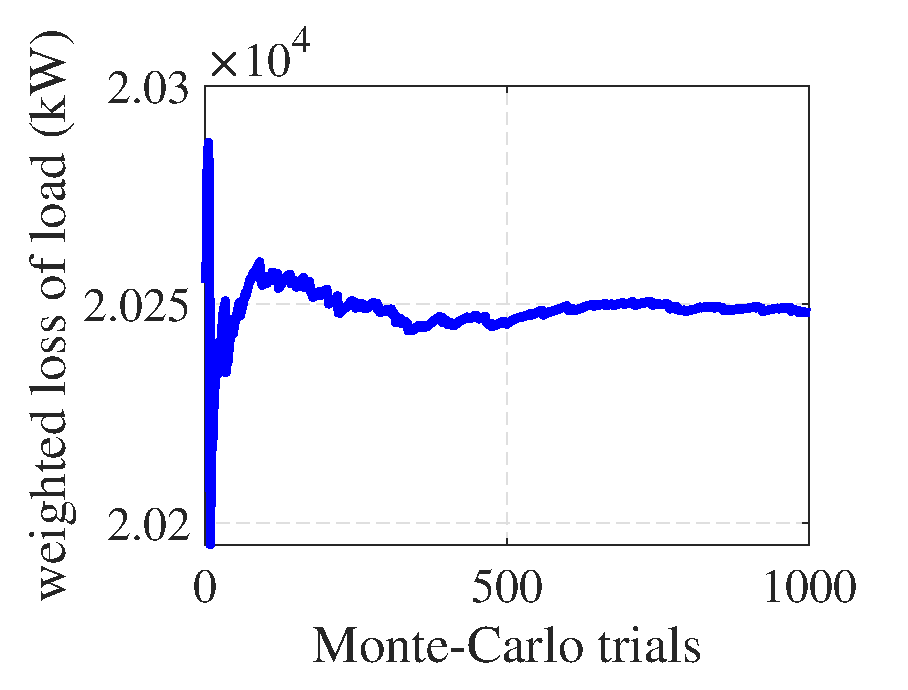
\includegraphics[width=0.42\linewidth]{figures/speed_40_MC_base.eps}
        \label{fig:MCS_2}
     }
     \caption{Moving average of loss of load obtained for 1000 Monte-Carlo trials a) without hardening when $u = 15~m/s$ and $p_f(u) = 0.002$ and b) with line hardening when $u = 40~m/s$ and $p_f(u) = 0.915$. For each wind speed scenario, it can be guaranteed that the prioritized load loss converges after 1000 Monte-Carlo trials.}
     \label{fig:MCS_convergence}
\end{figure}

\begin{figure}[h]
     \centering
    %  \subfigure[]
     {
%    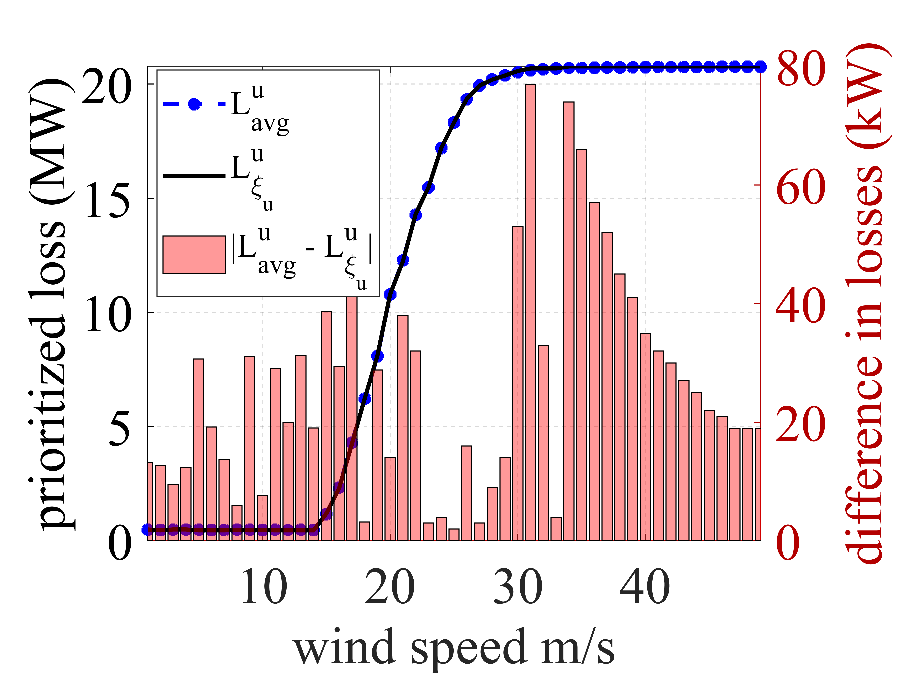
\includegraphics[width=0.42\linewidth]{figures/scenario_new_load_base.eps}
        \label{fig:scen_set_1}
    }\hfill
    % \subfigure[]
    {
%    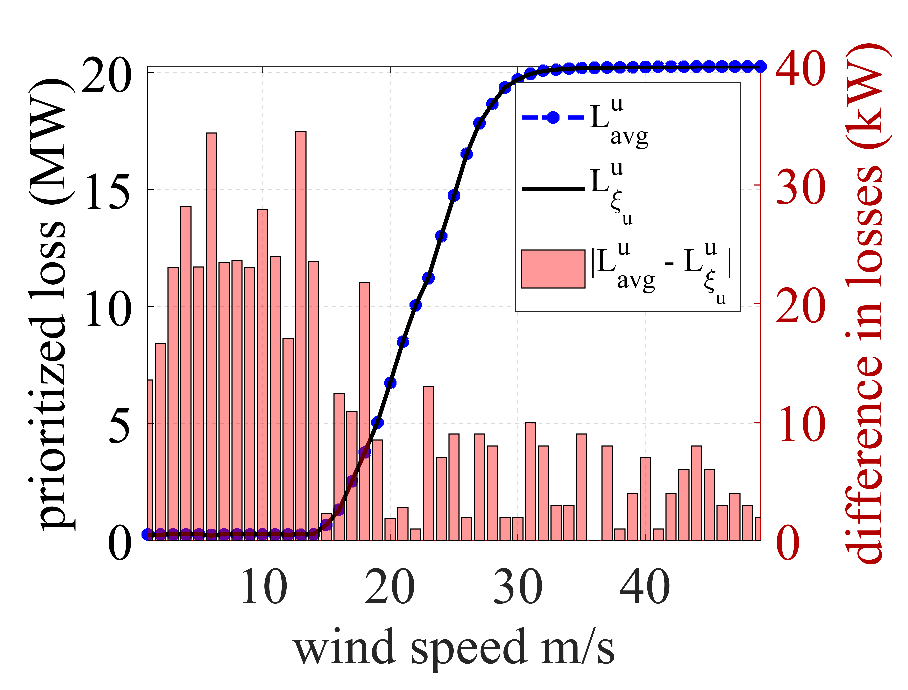
\includegraphics[width=0.42\linewidth]{figures/scenario_new_load_harden.eps}
        \label{fig:scen_set_2}
     }
     \caption{Comparison of prioritized load loss obtained for two sets of reduced scenarios a) without hardening b) with hardening.}
     \label{fig:scenario_reduction}
\end{figure}

\paragraph{Risk-based Planning}
In this long-term planning problem, 6 DG locations are pre-selected as potential locations for the placement of DG units. The selected potential DG locations are nodes 95, 122, 39, 85, 56, and 66. However, the DG locations are decided by the optimization model and $\delta_i^{DG} = 1$ if and only if $\beta_i^{DG} > 0$. From the operator's perspective, it is often practical to have a limited budget while planning the siting and sizing strategies for DGs. The total budget is constrained so that the sum of the DG units is less than or equal to 900 kW.  For risk-driven problems, $\alpha$ is set at 0.95, meaning that 5\% tail scenarios (HILP) are considered to have greater risks.

\begin{table}[t]
    \centering
    \caption{Base case expected value and $CVaR_\alpha$ of prioritized load loss.}
    \begin{tabular}{|c|c|c|c|}
    \hline
          line hardening & $\mathbb{E}(Q(\delta, \mathcal{E}))$ in kW & $CVaR_\alpha(Q(\delta, \mathcal{E}))$ in kW \\
    \hline
         No & 5982.57  & 20601.58  \\
    \hline
         Yes & 4541.76  & 19839.39 \\ 
    \hline
    \end{tabular}
    \label{tab:base_case}
\end{table}

\begin{table}
    \centering
    \caption{Expected value and $CVaR_\alpha$ of prioritized load loss and prioritized critical load (PCL) picked up for different values of $\lambda$. The DG planning strategy differs along with the risk preference defined by $\lambda$. All of the values mentioned here are in kW.}
    \begingroup
    \setlength{\tabcolsep}{5pt} % Default value: 6pt
    \renewcommand{\arraystretch}{1.5}
    \begin{adjustbox}{width=1\textwidth,center=1\textwidth}
    \color{black}{
    \begin{tabular}{|c!{\vrule width 1.5pt}c|c|c!{\vrule width 1.5pt}c|c|c!{\vrule width 1.5pt}c|c|c!{\vrule width 1.5pt}c|c|c!{\vrule width 1.5pt}c|c|c!{\vrule width 1.5pt}c|c|c!{\vrule width 1.5pt}}
    \hline
       \multirow{2}{*}{} & \multicolumn{9}{c!{\vrule width 1.5pt}}{\textbf{WITHOUT LINE HARDENING}} & \multicolumn{9}{c!{\vrule width 1.5pt}}{\textbf{WITH LINE HARDENING}} \\
   \hline
        \multirow{2}{*}{} & \multicolumn{3}{c!{\vrule width 1.5pt}}{\makecell{Existing methods\\~\cite{8329529, 2021IASTATE, 9136725}}} & \multicolumn{6}{c!{\vrule width 1.5pt}}{Proposed method} & \multicolumn{3}{c!{\vrule width 1.5pt}}{\makecell{Existing methods\\~\cite{8329529, 2021IASTATE, 9136725}}} & \multicolumn{6}{c!{\vrule width 1.5pt}}{Proposed method} \\
    
    \cline{2-19}
           & \multicolumn{3}{c!{\vrule width 1.5pt}}{$\bm{\lambda = 0}$} & \multicolumn{3}{c!{\vrule width 1.5pt}}{$\bm{\lambda = 0.5}$} & \multicolumn{3}{c!{\vrule width 1.5pt}}{$\bm{\lambda = 1}$}& \multicolumn{3}{c!{\vrule width 1.5pt}}{$\bm{\lambda = 0}$} & \multicolumn{3}{c!{\vrule width 1.5pt}}{$\bm{\lambda = 0.5}$} & \multicolumn{3}{c!{\vrule width 1.5pt}}{$\bm{\lambda = 1}$} \\
    \hline
         $\mathbb{E}(Q(\delta,\mathcal{E}))$ & \multicolumn{3}{c!{\vrule width 1.5pt}}{3567.12} & \multicolumn{3}{c!{\vrule width 1.5pt}}{3586.28} & \multicolumn{3}{c!{\vrule width 1.5pt}}{3595.51} & \multicolumn{3}{c!{\vrule width 1.5pt}}{2467.46} & \multicolumn{3}{c!{\vrule width 1.5pt}}{2463.95} & \multicolumn{3}{c!{\vrule width 1.5pt}}{2490.09} \\ 
    \hline
        $CVaR_{\alpha}(Q(\delta,\mathcal{E}))$ & \multicolumn{3}{c!{\vrule width 1.5pt}}{19093.89} & \multicolumn{3}{c!{\vrule width 1.5pt}}{18885.92} & \multicolumn{3}{c!{\vrule width 1.5pt}}{18885.92} & \multicolumn{3}{c!{\vrule width 1.5pt}}{18415.04} & \multicolumn{3}{c!{\vrule width 1.5pt}}{18160.18} & \multicolumn{3}{c!{\vrule width 1.5pt}}{18119.1} \\
    \hline
         \makecell{Expectation of PCL\\ picked up} & \multicolumn{3}{c!{\vrule width 1.5pt}}{15043.93} & \multicolumn{3}{c!{\vrule width 1.5pt}}{15016.64} & \multicolumn{3}{c!{\vrule width 1.5pt}}{15006.62} & \multicolumn{3}{c!{\vrule width 1.5pt}}{16065.76} & \multicolumn{3}{c!{\vrule width 1.5pt}}{16048.17} & \multicolumn{3}{c!{\vrule width 1.5pt}}{16026.12} \\ 
    \hline
        \makecell{$CVaR_{\alpha}$ of PCL\\ picked up} & \multicolumn{3}{c!{\vrule width 1.5pt}}{3406.59} & \multicolumn{3}{c!{\vrule width 1.5pt}}{3603.06} & \multicolumn{3}{c!{\vrule width 1.5pt}}{3603.06} & \multicolumn{3}{c!{\vrule width 1.5pt}}{4953.65} & \multicolumn{3}{c!{\vrule width 1.5pt}}{5580.72} & \multicolumn{3}{c!{\vrule width 1.5pt}}{6295.33}  \\
    \hline
        \multirow{4}{*}{\makecell{DG planning \\strategies}} & $\bm{\beta^{DG}_{39}}$ & $\bm{\beta^{DG}_{56}}$ & $\bm{\beta^{DG}_{66}}$ & $\bm{\beta^{DG}_{39}}$ & $\bm{\beta^{DG}_{56}}$ & $\bm{\beta^{DG}_{66}}$ & $\bm{\beta^{DG}_{39}}$ & $\bm{\beta^{DG}_{56}}$ & $\bm{\beta^{DG}_{66}}$ & $\bm{\beta^{DG}_{39}}$ & $\bm{\beta^{DG}_{56}}$ & $\bm{\beta^{DG}_{66}}$ & $\bm{\beta^{DG}_{39}}$ & $\bm{\beta^{DG}_{56}}$ & $\bm{\beta^{DG}_{66}}$ & $\bm{\beta^{DG}_{39}}$ & $\bm{\beta^{DG}_{56}}$ & $\bm{\beta^{DG}_{66}}$   \\   
        \cline{2-19}
        & 0 & 20 & 370 & 20 & 20 & 340 & 20 & 20 & 370 & 0 & 350 & 330 & 20 & 220 & 255 & 20 & 170 & 330 \\
    \cline{2-19}
        & $\bm{\beta^{DG}_{85}}$ & $\bm{\beta^{DG}_{95}}$ & $\bm{\beta^{DG}_{122}}$ & $\bm{\beta^{DG}_{85}}$ & $\bm{\beta^{DG}_{95}}$ & $\bm{\beta^{DG}_{122}}$ & $\bm{\beta^{DG}_{85}}$ & $\bm{\beta^{DG}_{95}}$ & $\bm{\beta^{DG}_{122}}$ & $\bm{\beta^{DG}_{85}}$ & $\bm{\beta^{DG}_{95}}$ & $\bm{\beta^{DG}_{122}}$ & $\bm{\beta^{DG}_{85}}$ & $\bm{\beta^{DG}_{95}}$ & $\bm{\beta^{DG}_{122}}$ & $\bm{\beta^{DG}_{85}}$ & $\bm{\beta^{DG}_{95}}$ & $\bm{\beta^{DG}_{122}}$ \\
    \cline{2-19}
        & 390 & 0 & 120 & 100 & 300 & 120 & 100 & 270 & 120 & 100 & 0 & 120 & 100 & 305 & 0 & 100 & 280 & 0 \\
    \hline
    \end{tabular}}
    \end{adjustbox}
    \endgroup
    \label{tab:result_first_case}
\end{table}

To identify the trade-off among different DG-based planning strategies, 6 locations --- 39, 56, 66, 85, 95, and 122 --- are selected as potential DG locations. First, we discuss the results for the risk-neutral case ($\lambda=0$). The existing resilience-based planning methods,~\cite{8329529, 2021IASTATE, 9136725}, are focused on the risk-neutral case and used as a comparison for this work. The overall capacity of each of the DGs is shown in Table~\ref{tab:result_first_case}. For risk-neutral planning without line hardening measures, no DGs are required to be placed on nodes 36 and 95. However, for mean-risk and risk-averse situations, the planning strategies change significantly. For risk-involved strategies, it is required to place DGs on nodes 39 and 95 while reducing the DG sizes for the rest of the nodes as shown in Table~\ref{tab:result_first_case}. Hence, the trade-off of including risk minimization in the objective is to increase the number of DG units in the system. This can be fruitful for extreme event scenarios when picking up some of the CLs is required, even though it increases the expected value of prioritized load loss. Table~\ref{tab:result_first_case} also shows the expected value and $CVaR_\alpha$ of prioritized CLs picked up by different planning strategies. It can be seen that the expected value of prioritized CLs picked up does not change much regardless of the risk preference. However, for risk-based strategies (both mean risk and risk-averse), $CVaR_\alpha$ of prioritized CLs picked up increases by $200~kW$ compared to the risk-neutral case. 

The effect of risk aversion is even more pronounced in the case with the line-hardening strategy. Fig.~\ref{fig:neutral_vs_averse_harden} shows a restoration and planning solution for a specific scenario of HILP nature, $u = 28~m/s$. The lines and nodes with black color are the energized section, whereas non-energized sections are represented by gray. Similarly, red lines represent out-of-service lines due to the particular outage scenario.
Similar to the restoration for cases without line hardening measures, the risk-neutral solution does not include DGs in nodes 39 and 95. When the objective is risk-neutral ($\lambda=0$) some of the prioritized critical loads are not picked up in this specific scenario as picking up critical loads in this scenario would not affect the expected value of load served for the overall scenarios. Since the objective is to minimize the expected value of prioritized load loss for entire scenarios, DG at location 95 is not selected. Note that the probability of HILP scenarios is low. Since the expected value contains the product of this probability with the objective function in the restoration phase, the net value is significantly low to affect the overall expected value. However, when the objective is risk-averse, any prioritized load that the nearest possible DG can pick up is given the top priority for any HILP event. For instance, it can be seen that load at node 62 is picked up by DG at node 95 through path 95-93-94-54-57-60-62.
Hence, this draws an important conclusion that risk-averse decisions enhance long-term resilience planning by focusing the extreme HILP events. Contrary to the existing methods in~\cite{8329529, 2021IASTATE, 9136725}, the prioritized CLs have a high chance of being picked up when an HILP event is realized by including risk minimization in the objective. However, when attempting to minimize the risk-averse objective (i.e., the $CVaR_\alpha$), we incur an additional DG cost in the overall planning budget to meet the requirements for risk-averse planning. Thus, through the proposed approach and by including $CVaR_\alpha$ minimization in the objective function, prioritized critical loads can be properly restored in case of HILP events. Furthermore, with the changing trade-off between the expectation and the $CVaR_\alpha$ of the prioritized load loss, the expected value \textit{generally} decreases with the increase in $\lambda$. 

\begin{figure}[ht]
        \centering
        % \subfigure[]
        {
%    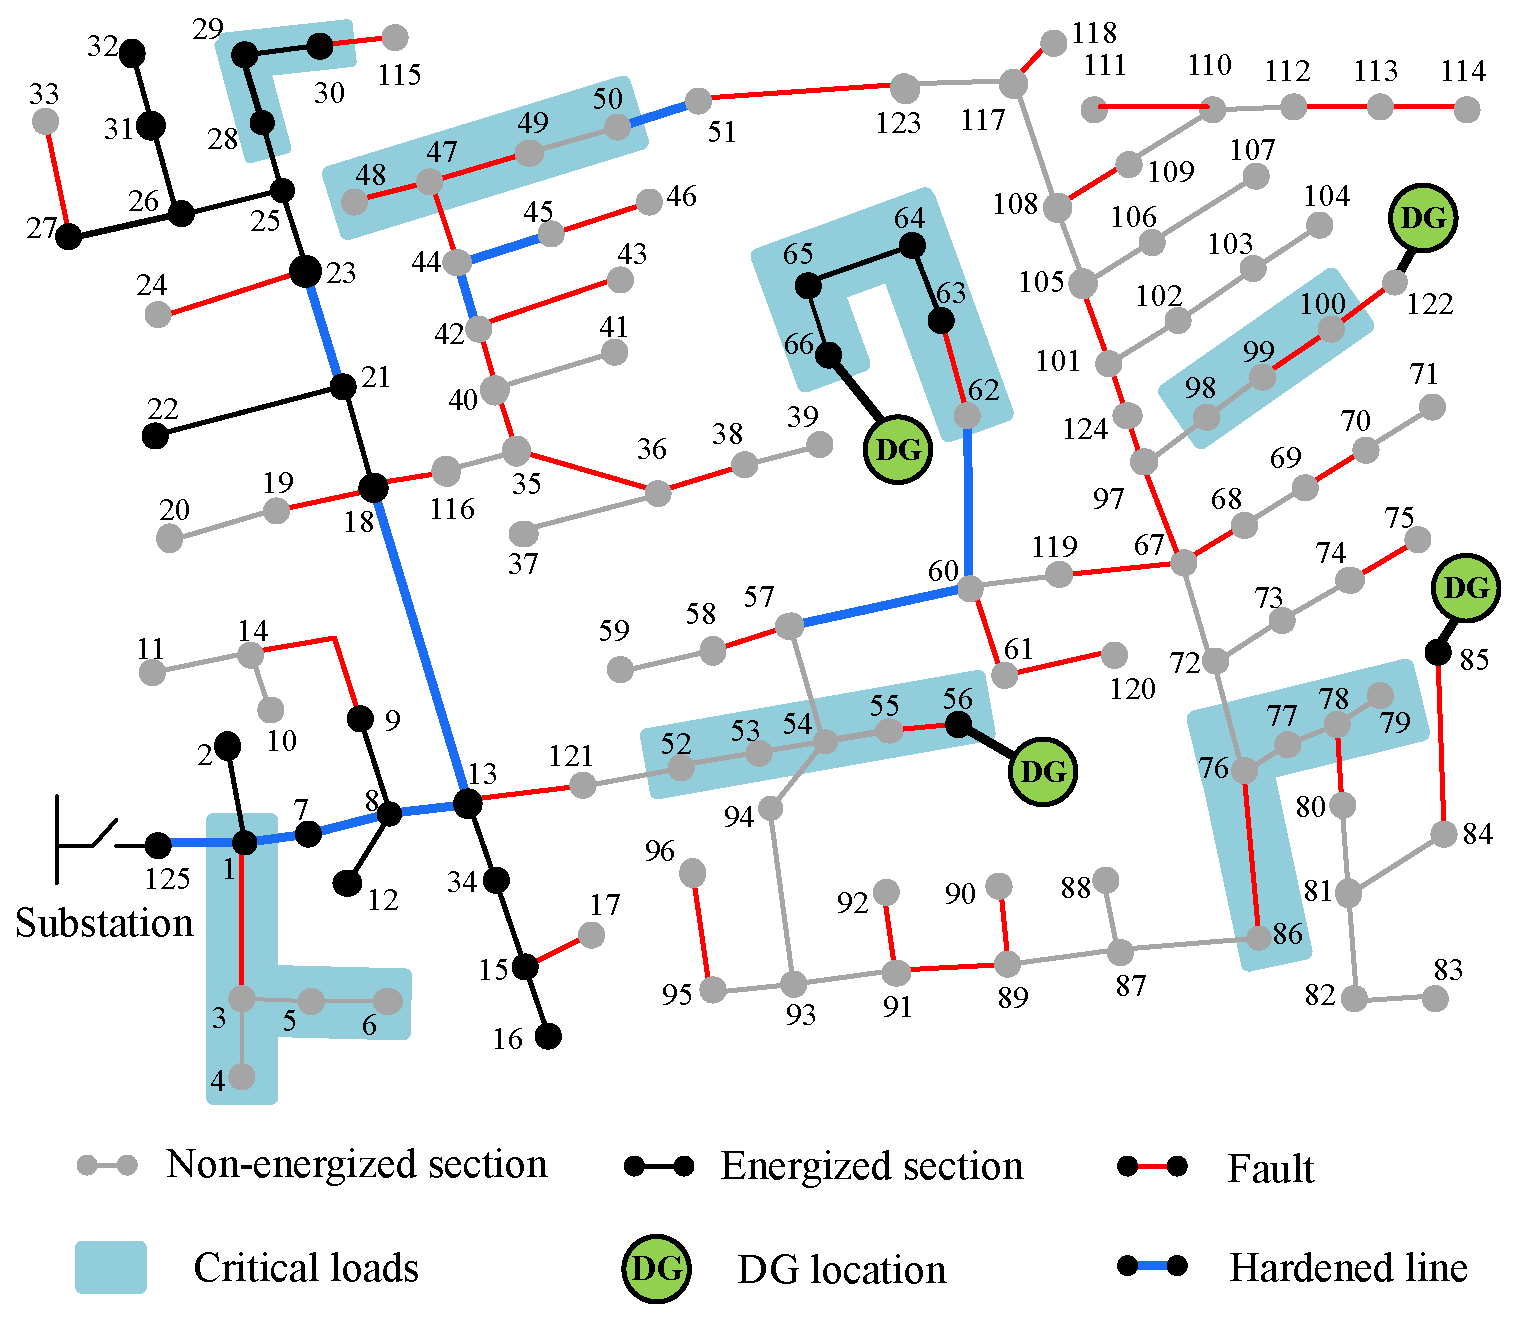
\includegraphics[width=0.48\textwidth]{figures/harden_neutral.eps}
    }\hfill
    % \subfigure[]
    {
%    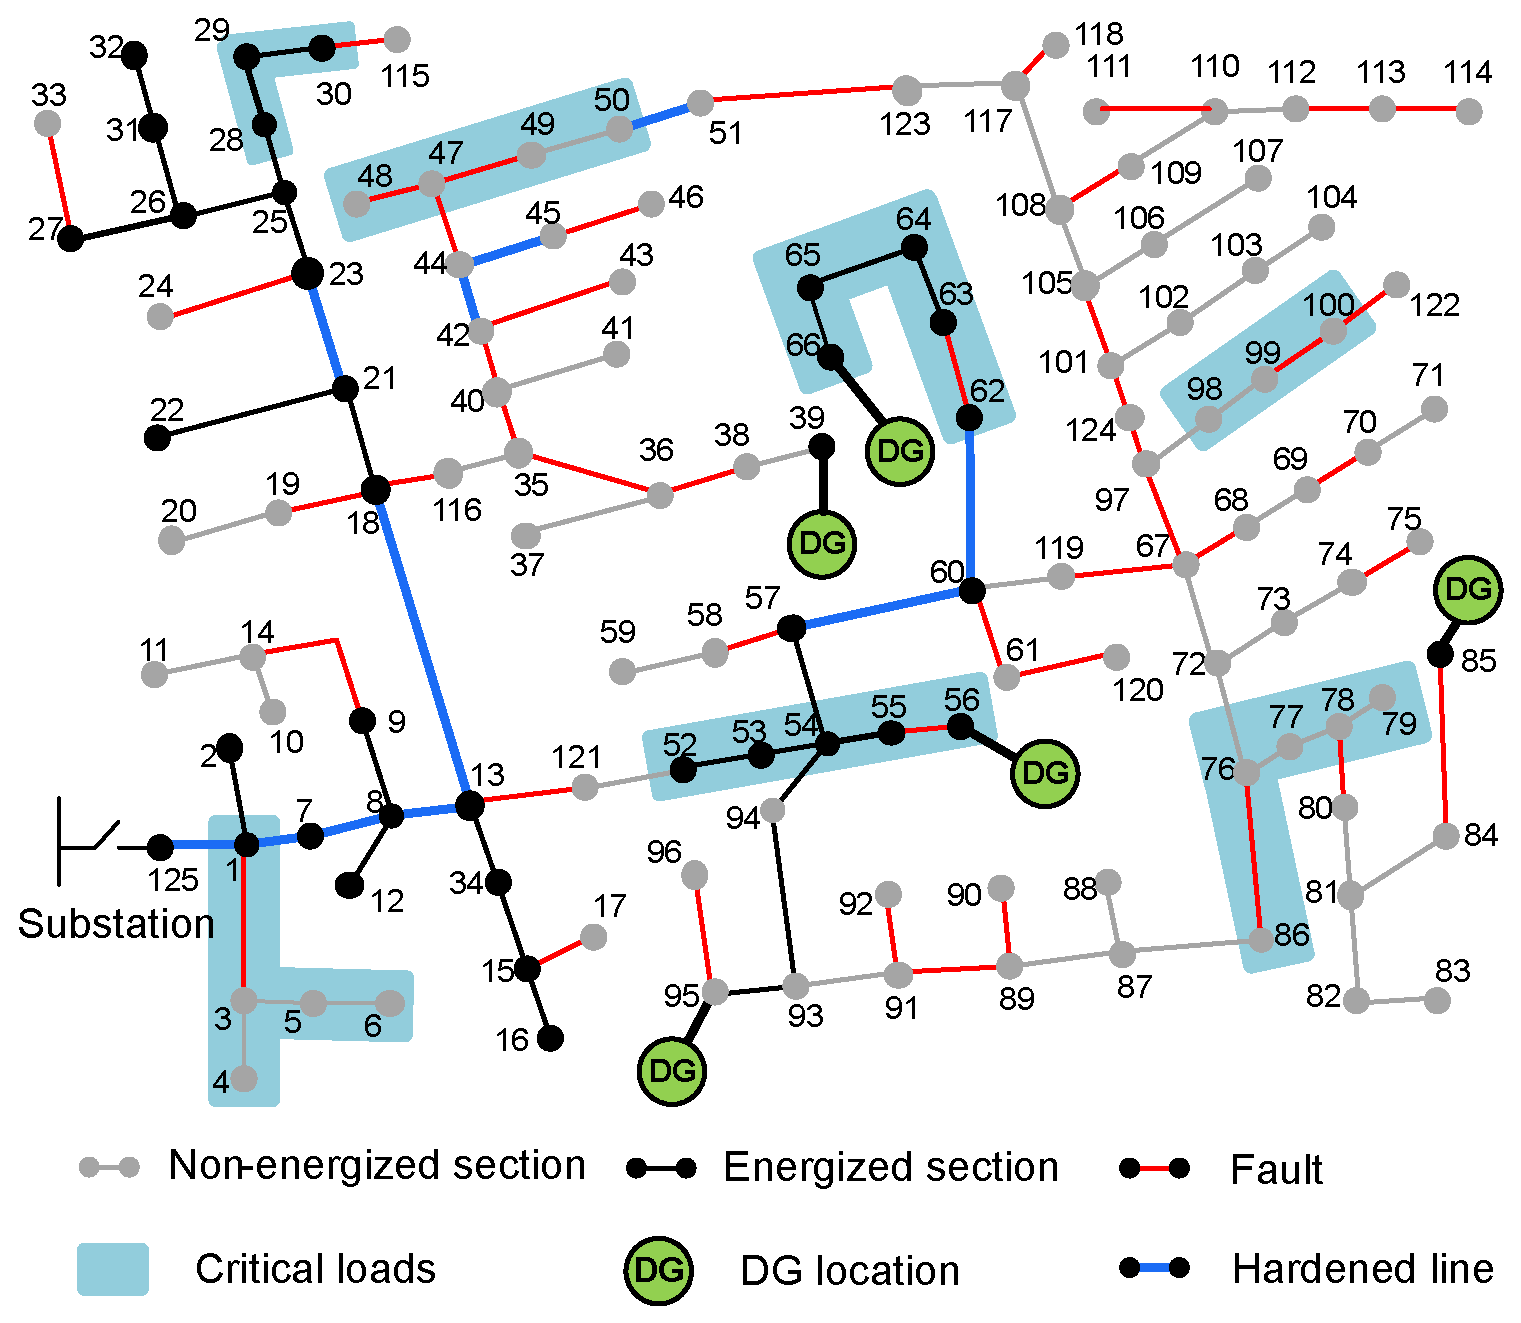
\includegraphics[width=0.48\textwidth]{figures/harden_averse.eps}  
     }
    \caption{\revise{DG sizing and siting solution for a specific scenario with additional hardening measures for a) risk-neutral and b) risk-averse planning strategy.}}
    \label{fig:neutral_vs_averse_harden}
\end{figure}

\paragraph{Sensitivity Analysis}
The value of $CVaR$ depends on several factors such as investment decisions, budget, risk preference, and scenarios under consideration. Here, we present a few of the sensitivity analyses and discuss their impacts on $CVaR$. For simplicity, the analyses are performed only on the system with additional hardening measures already in place and for sensitivity based on time complexity, the analysis is done in terms of expected value of the second stage.

\begin{figure}[t]
    \centering
%    \includegraphics[width=0.8\textwidth]{figures/CVaR_alpha_harden.eps}
    \vspace{-0.6cm}
    \caption{Comparison of $CVaR_\alpha$ of prioritized loss of load for different values of $\alpha$ and risk preference.}
    \label{fig:CVaR_vs_alpha}
\end{figure}

\begin{figure}[!ht]
     \centering
    %  \subfigure[]
     {
%    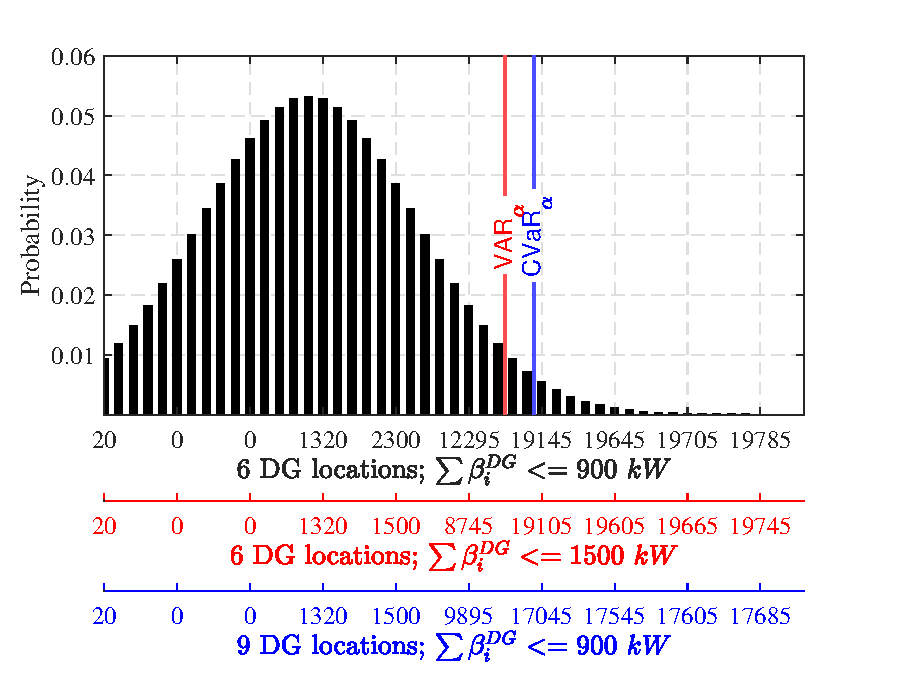
\includegraphics[width=0.7\textwidth]{figures/DG_tradeoff_neutral.eps}
        \label{fig:DG_neutral}
    }
    % \subfigure[]
    {
%    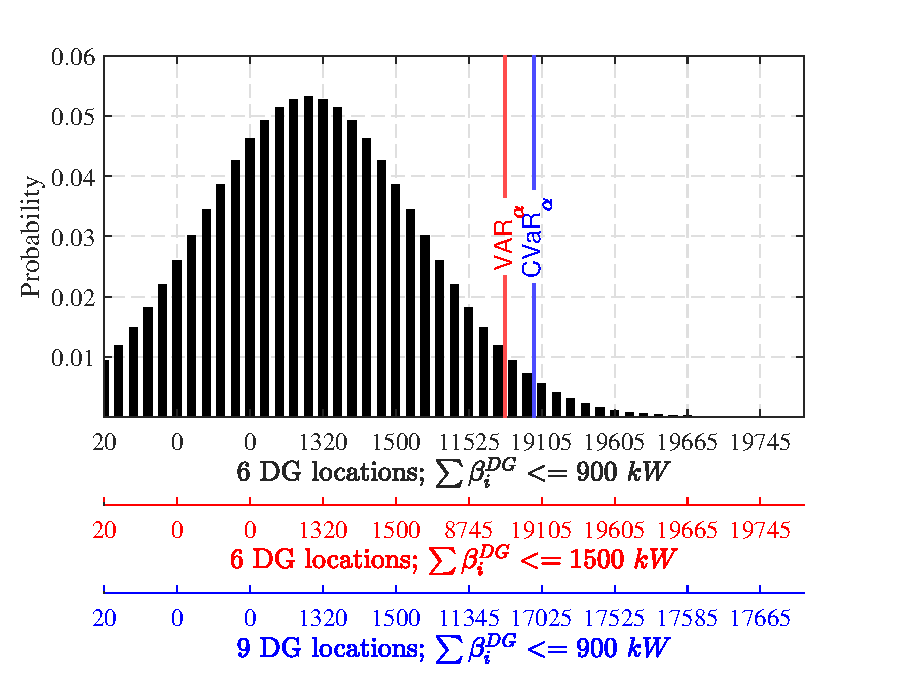
\includegraphics[trim ={0 0 0 0.5cm} ,clip, width=0.7\textwidth]{figures/DG_tradeoff_averse.eps}
        \label{fig:DG_averse}
     }
     \caption{$CVaR_\alpha$ for different DG investment strategies for a) risk-neutral and b) risk-averse planning. The value on the x-axis represents the prioritized loss of load for each $\xi$ with corresponding $p_\xi$ represented on the y-axis.}
     \label{fig:DG_tradeoffs}
     \vspace{-0.4cm}
\end{figure}

\begin{figure*}[!t]
        \centering
        % \vspace{0.5 cm}
%    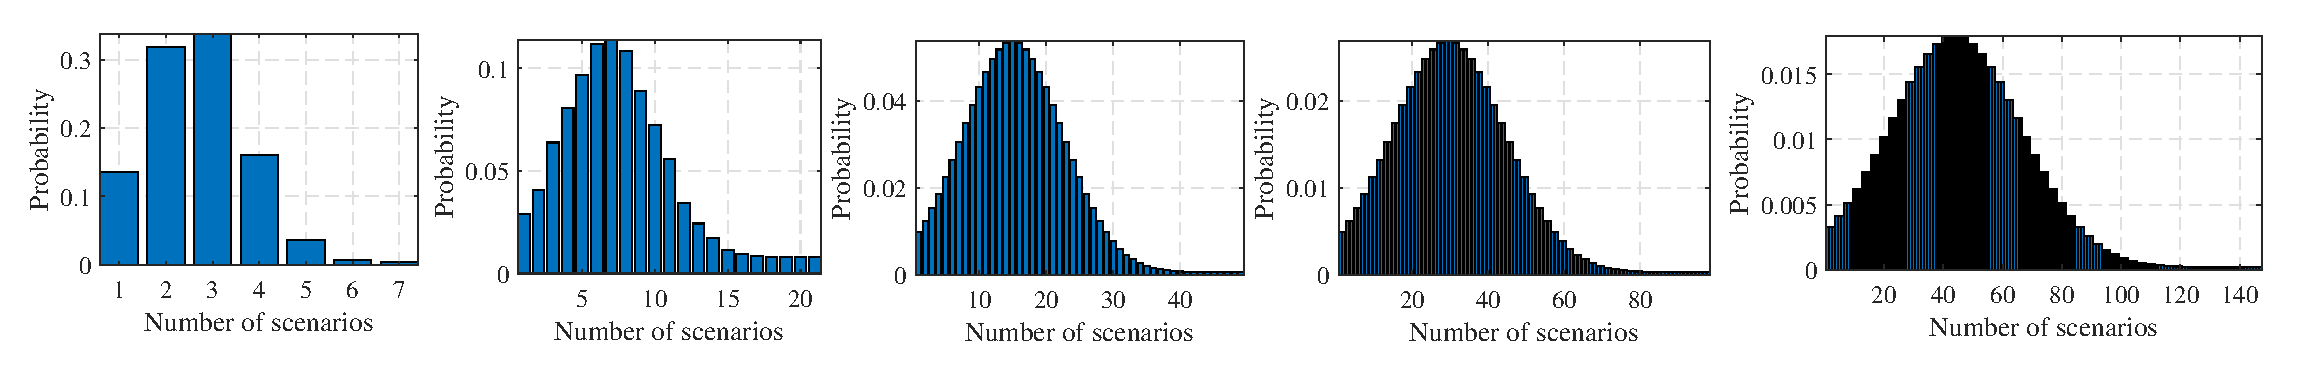
\includegraphics[width=\textwidth]{figures/different_scenarios_2.eps}
        \caption{\revise{Different number of scenarios with respective probabilities of occurrence: (a) 7 scenarios, (b) 21 scenarios; (c) 49 scenarios, (d) 98 scenarios e) 147 scenarios.}}
        \label{fig:scen_probab}
\end{figure*}

\paragraph{Change in confidence level}
The risk parameters $\alpha$ and $\lambda$ can affect the planning decisions. The value of $CVaR_\alpha$ highly depends on $\alpha$ as it defines the number of scenarios to be considered in defining the risk. In other words, $\alpha$ can also be defined as risk percentage. For a higher value of $\alpha$, the value of $VAR_\alpha$ increases, and hence, $CVaR_\alpha$ represents the scenarios that create greater losses in the system. Similarly, for a smaller $\alpha$, $CVaR_\alpha$ incorporates a larger number of scenarios with lower losses in risk quantification. Furthermore, as discussed above, an increasing value of $\lambda$ denotes an increase in risk aversion towards planning decisions. Fig.~\ref{fig:CVaR_vs_alpha} shows the relation of $CVaR_\alpha$ for the prioritized loss of load for different values of $\lambda$ and $\alpha$. As discussed, $CVaR_\alpha$ decreases when more scenarios are considered as risky (characterized by $\alpha$). Furthermore, for a fixed $\alpha$, $CVaR_\alpha$ decreases with the increase in the value of $\lambda$ as more importance are given to risk minimization. Appropriate values for $\alpha$ and $\lambda$ need to be selected based on planners' risk aversion criteria.

\paragraph{Change in investment strategies}
Changing investment strategies and allocating the budget properly can also affect the overall planning cost. First, the overall budget for DG sizing and installation is increased so that $\mathcal{C}^{DG}_{max}$ corresponds to $P_{DG}^{max} = 1500~kW$ for the same set of DGs and their potential locations. Secondly, 3 additional DG locations (47, 27, and 114) are identified as potential DG placement locations. Fig.~\ref{fig:DG_tradeoffs} shows the distribution of prioritized loss of load when different DG planning measures are taken for risk-neutral and risk-averse cases, respectively. It is interesting to notice that increasing the budget to increase the capacity of DGs has a limited effect on the $CVaR_\alpha$ minimization. However, the expected value of prioritized load loss decreases to $2222.43~kW$ from $2467.46~kW$. The conclusion is consistent for the risk-averse case. However, increasing the number of potential DG locations led to significant improvement in $CVaR_\alpha$ minimization. The change in expected loss is, however, insignificant. For the case with 9 potential DG locations, the value of $CVaR_\alpha$ decreases from $18415.04~kW$ to $16385.51~kW$, for the risk-neutral case, and from $18119.1~kW$ to $15811.59~kW$, for the risk-averse case. Thus, with a limited budget, multiple DG sites with smaller DGs are more effective in improving resilience. 

\paragraph{Change in number of scenarios and set of scenarios} 
Fig.~\ref{fig:scen_probab} shows five case studies simulated to evaluate the impacts of the number of scenarios (used in optimization) on solution quality and solve time; (a) 7 scenarios, (b) 21 scenarios, (c) 49 scenarios, (d) 98 scenarios, (e) 147 scenarios.  Hence, for each case, different scenario sets are obtained using the method discussed in Algorithm 1. Fig.~\ref{fig:scen_vs_time} shows the objective function value for the different number of scenarios (used in the optimization problem) along with the corresponding solve times. The result for each case is obtained by taking an average of 10 representative scenario sets closest to the average representative scenario. We can clearly observe the trade-off between the number of scenarios, solution quality, and solve time. When a higher number of scenarios are used in optimization, the solution quality improves; however, it also leads to a significant increase in the solve time. It is also interesting to note that the solution obtained for 49 scenarios (2719.17 kW) is very close to the one obtained for 147 scenarios (2764.16 kW). However, the solve time for the problem with 147 scenarios is 11 times greater than that with 49 scenarios. Hence, 49 scenarios work well from the point of view of solution as well as solve time as the additional number of scenarios increases the computational complexity with no significant improvement in the objective value.

\begin{figure}[!t!]
    \centering
%    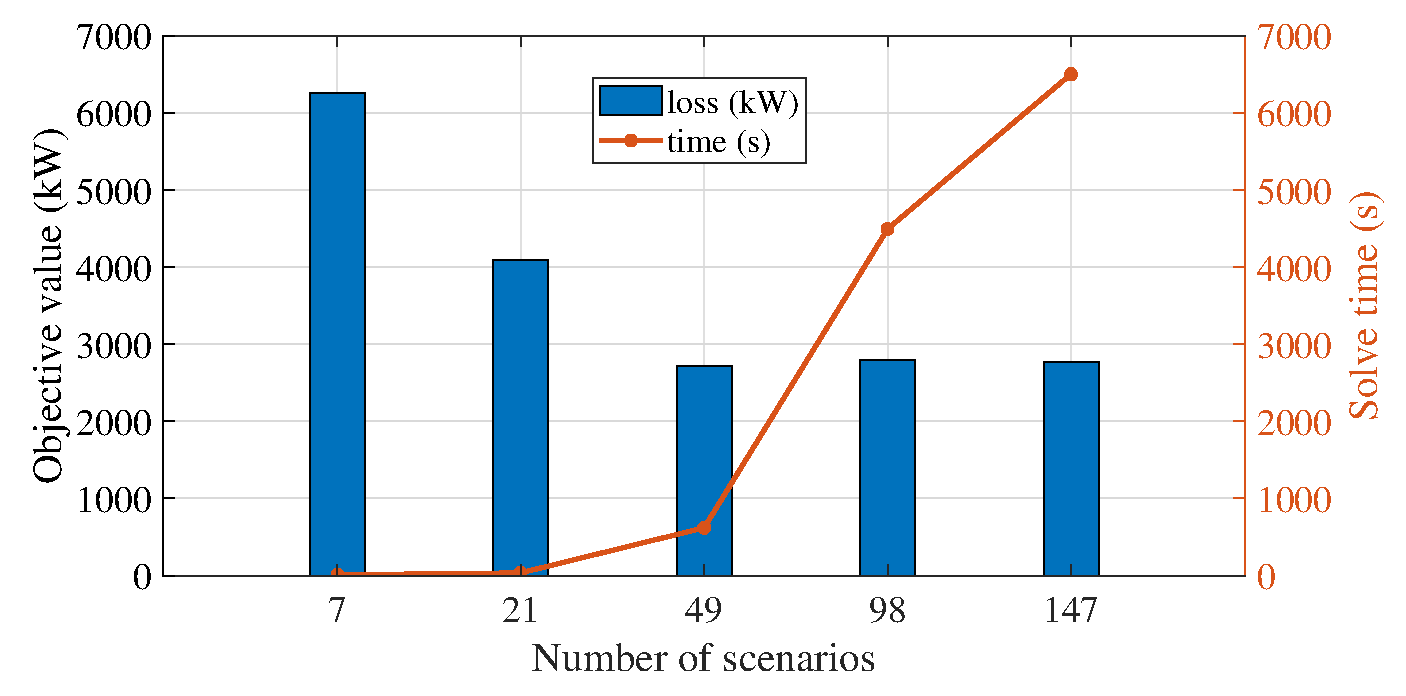
\includegraphics[width=0.7\textwidth]{figures/scenario_vs_time.eps}
    \caption{\revise{Comparison of objective value and solve time for a different number of scenarios.}}
    \label{fig:scen_vs_time}
\end{figure}

\begin{figure}[t]
    \centering
%    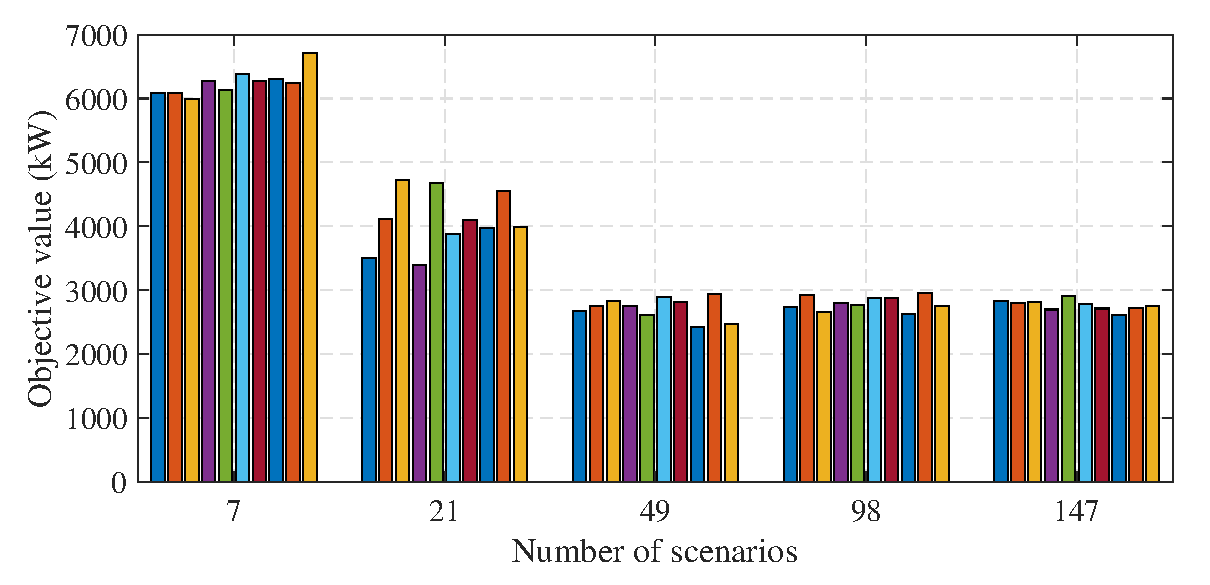
\includegraphics[width=0.7\textwidth]{figures/bundled_scenarios.eps}
    \caption{\revise{Comparison of objective value on a different set of scenarios for each number of scenarios sampled.}}
    \label{fig:scen_sets}
\end{figure}
